\chapter{Architecture} \fxnote{Hardware architecture - JH}
The architecture-chapters in the Rolling Road and AU2 documentations are made using SysML and UML. More specifically these languages are used to create BDDs (Block Definition Diagrams) and IBDs (Internal Block Diagram). These diagrams are included in the report - but for a complete explanation of these diagrams, the reader is referred to their corresponding documentations.\fxnote{reference til dokumentationer}

The diagrams are used help the reader gain a quick overview of the systems. Furthermore, the two types of diagrams are can be helpful to the developers in the following ways:
\begin{itemize}
	\item \textbf{BDD}\\
	To help define the function of the individual blocks and their boundaries. 
	\item \textbf{IBD}\\
	To help visualize how the different blocks should be connected and what their inputs and outputs are. By specifying the blocks' inputs and outputs in the initial work-phase, the design-phase becomes easier.
\end{itemize}

The BDD for AU2 is seen below in Figure \vref{fig:BDD_AU2}. This diagram has undergone several revisions before the team arrived at the version seen below. The first couple of revisions were much simpler as they contained fewer blocks. As the team began developing the blocks, however, it became clear that some blocks needed to be split up in order to maintain simplicity. Due to the flexibility of SCRUM this could easily be done.

In theory this kind of architecture would lead to a work-phase where every block can be designed independently from each other and then simply be connected in the end.

The IBD for AU2 is also seen below in Figure \vref{fig:IBD_AU2}. In order to maintain coherency between the BDD and IBD this diagram was being revised parallel with the BDD. Many of the signals seen in the IBD were also omitted in the first drafts - but added later as the development went under way it became clear that they were needed to make a functional system.

Some of the more complex systems are the Battery Management System and the Motor Control System. These systems are too complex, so they required individual IBDs to explain properly and thus creating a 'layered IDB'. These IBDs are omitted from this report - but is available in the documentation \fxnote{reference}.


\newpage
\begin{figure}[H]
	\centering
	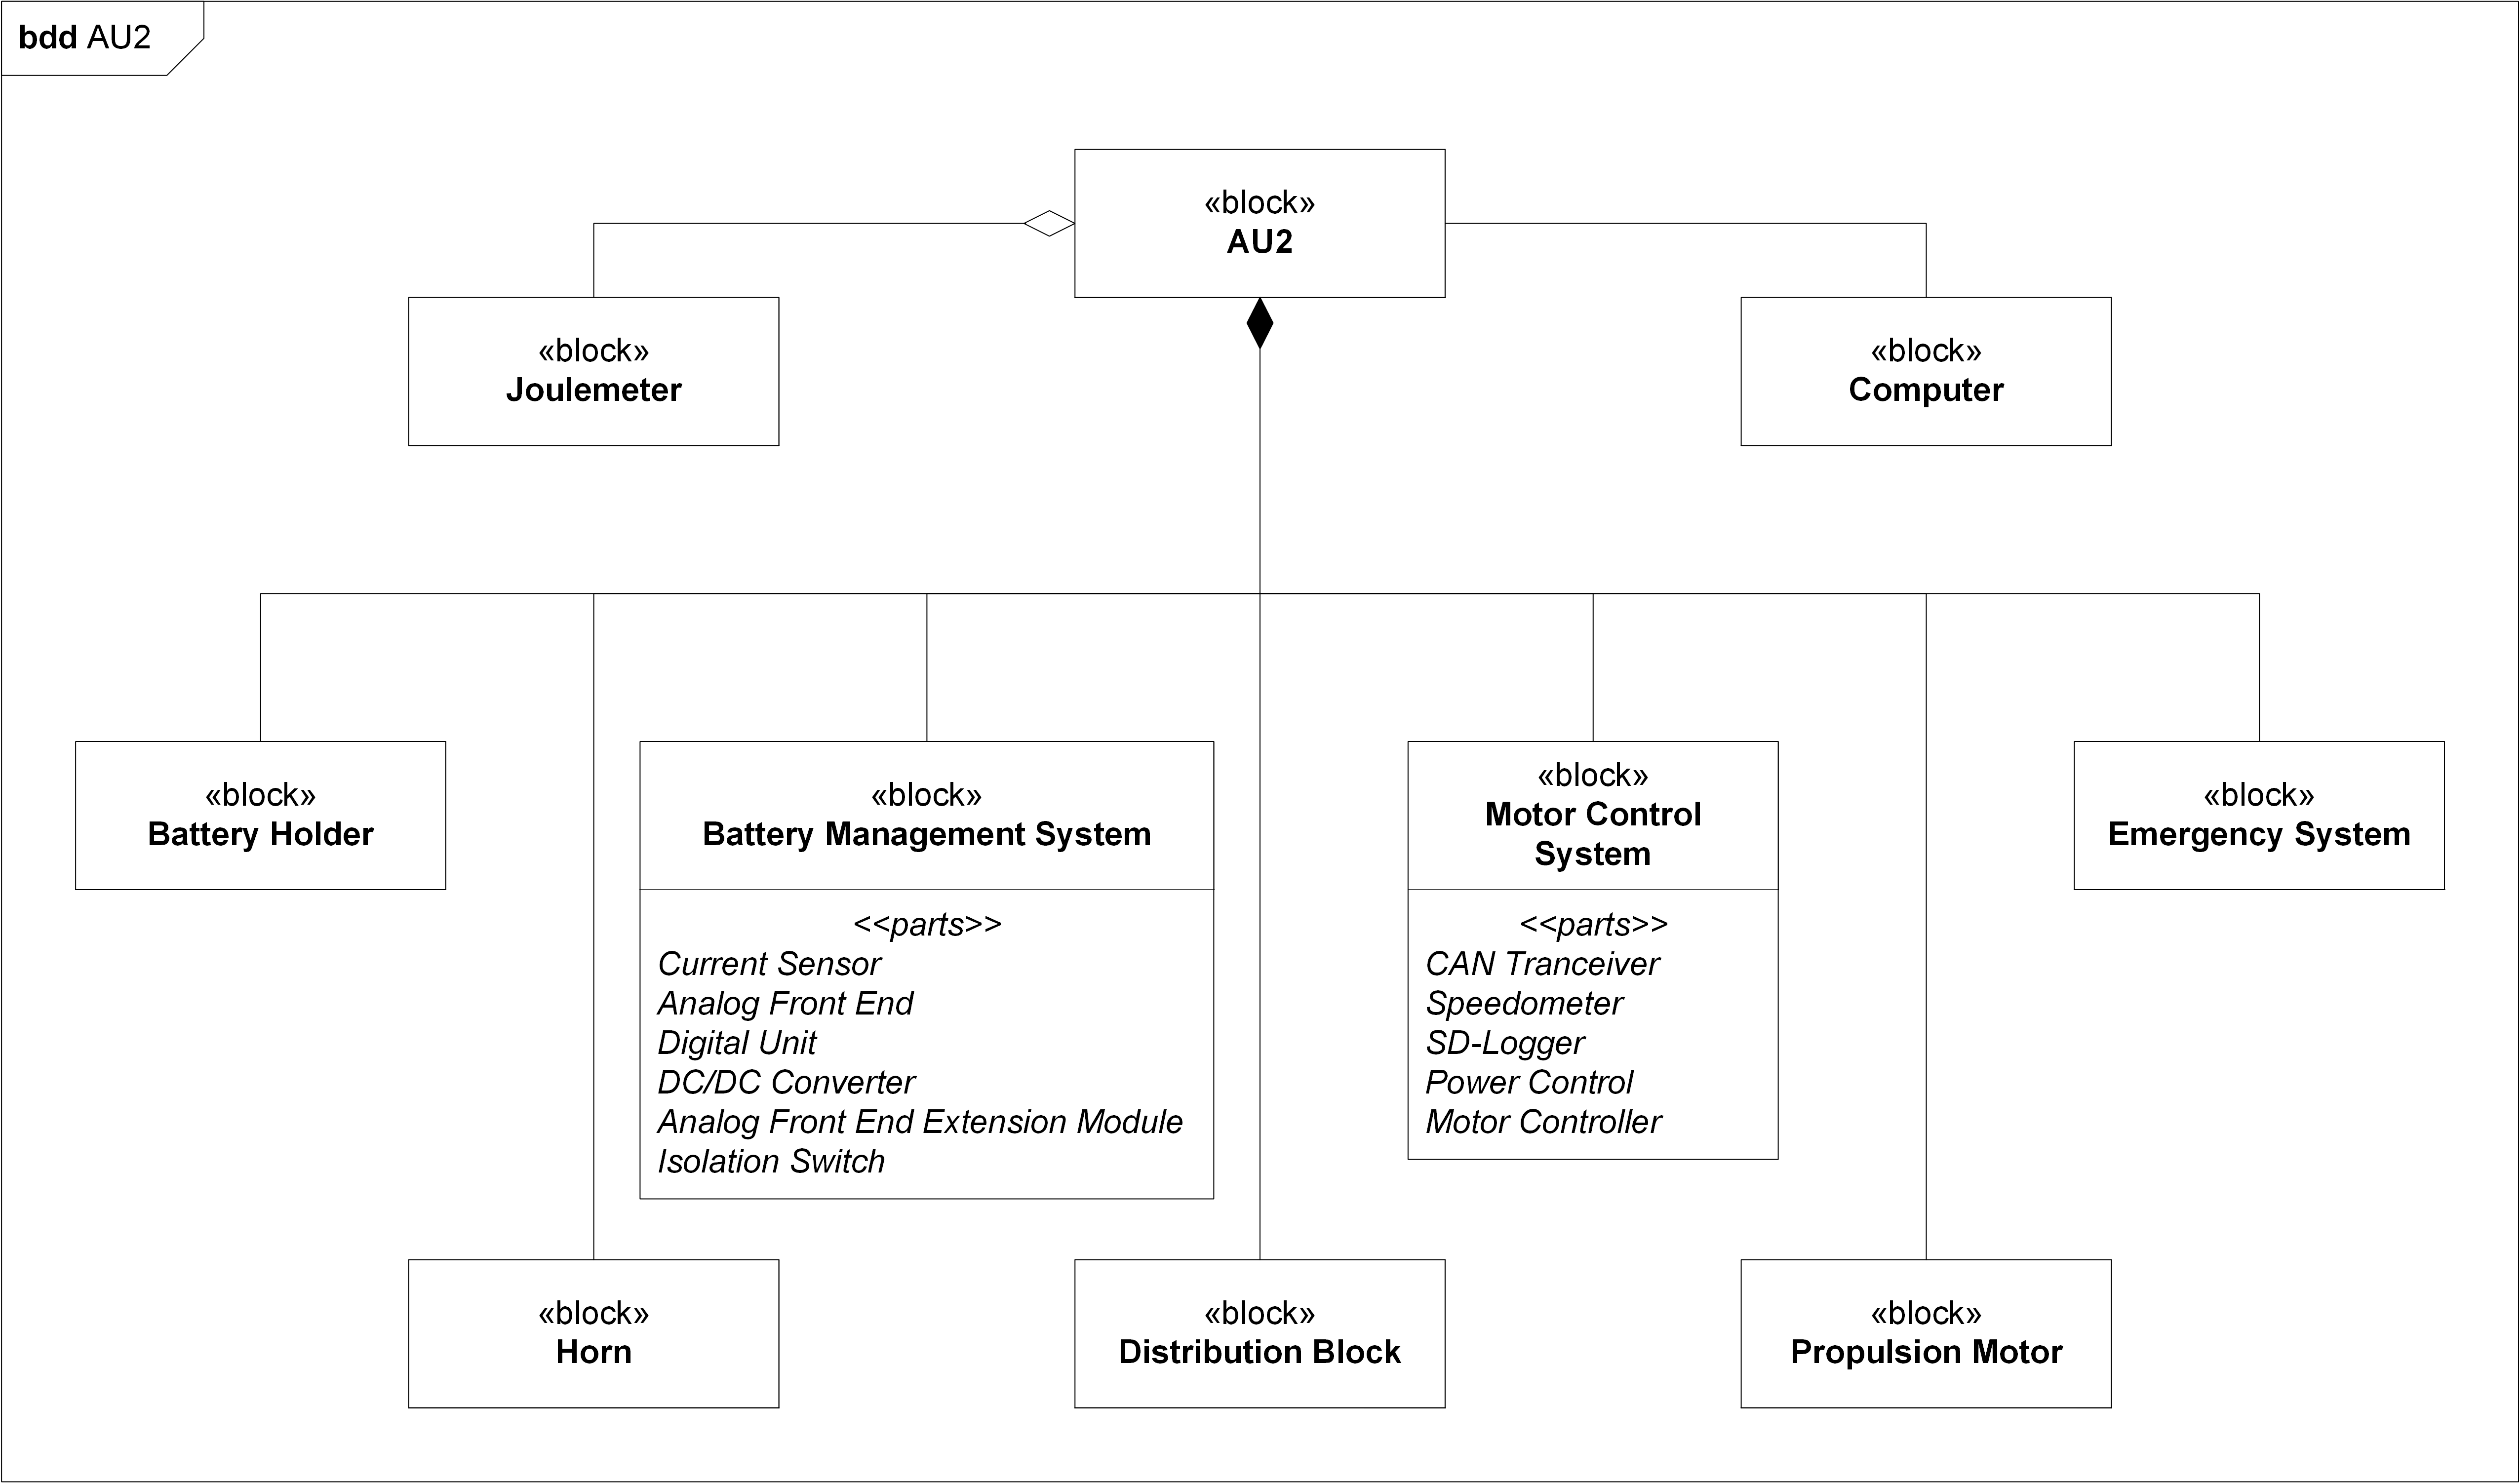
\includegraphics[width=1\linewidth]{Architecture/BDD_AU2}
	\caption{Block Definition Diagram for AU2}
	\label{fig:BDD_AU2}
\end{figure}

\begin{figure}[H]
	\centering
	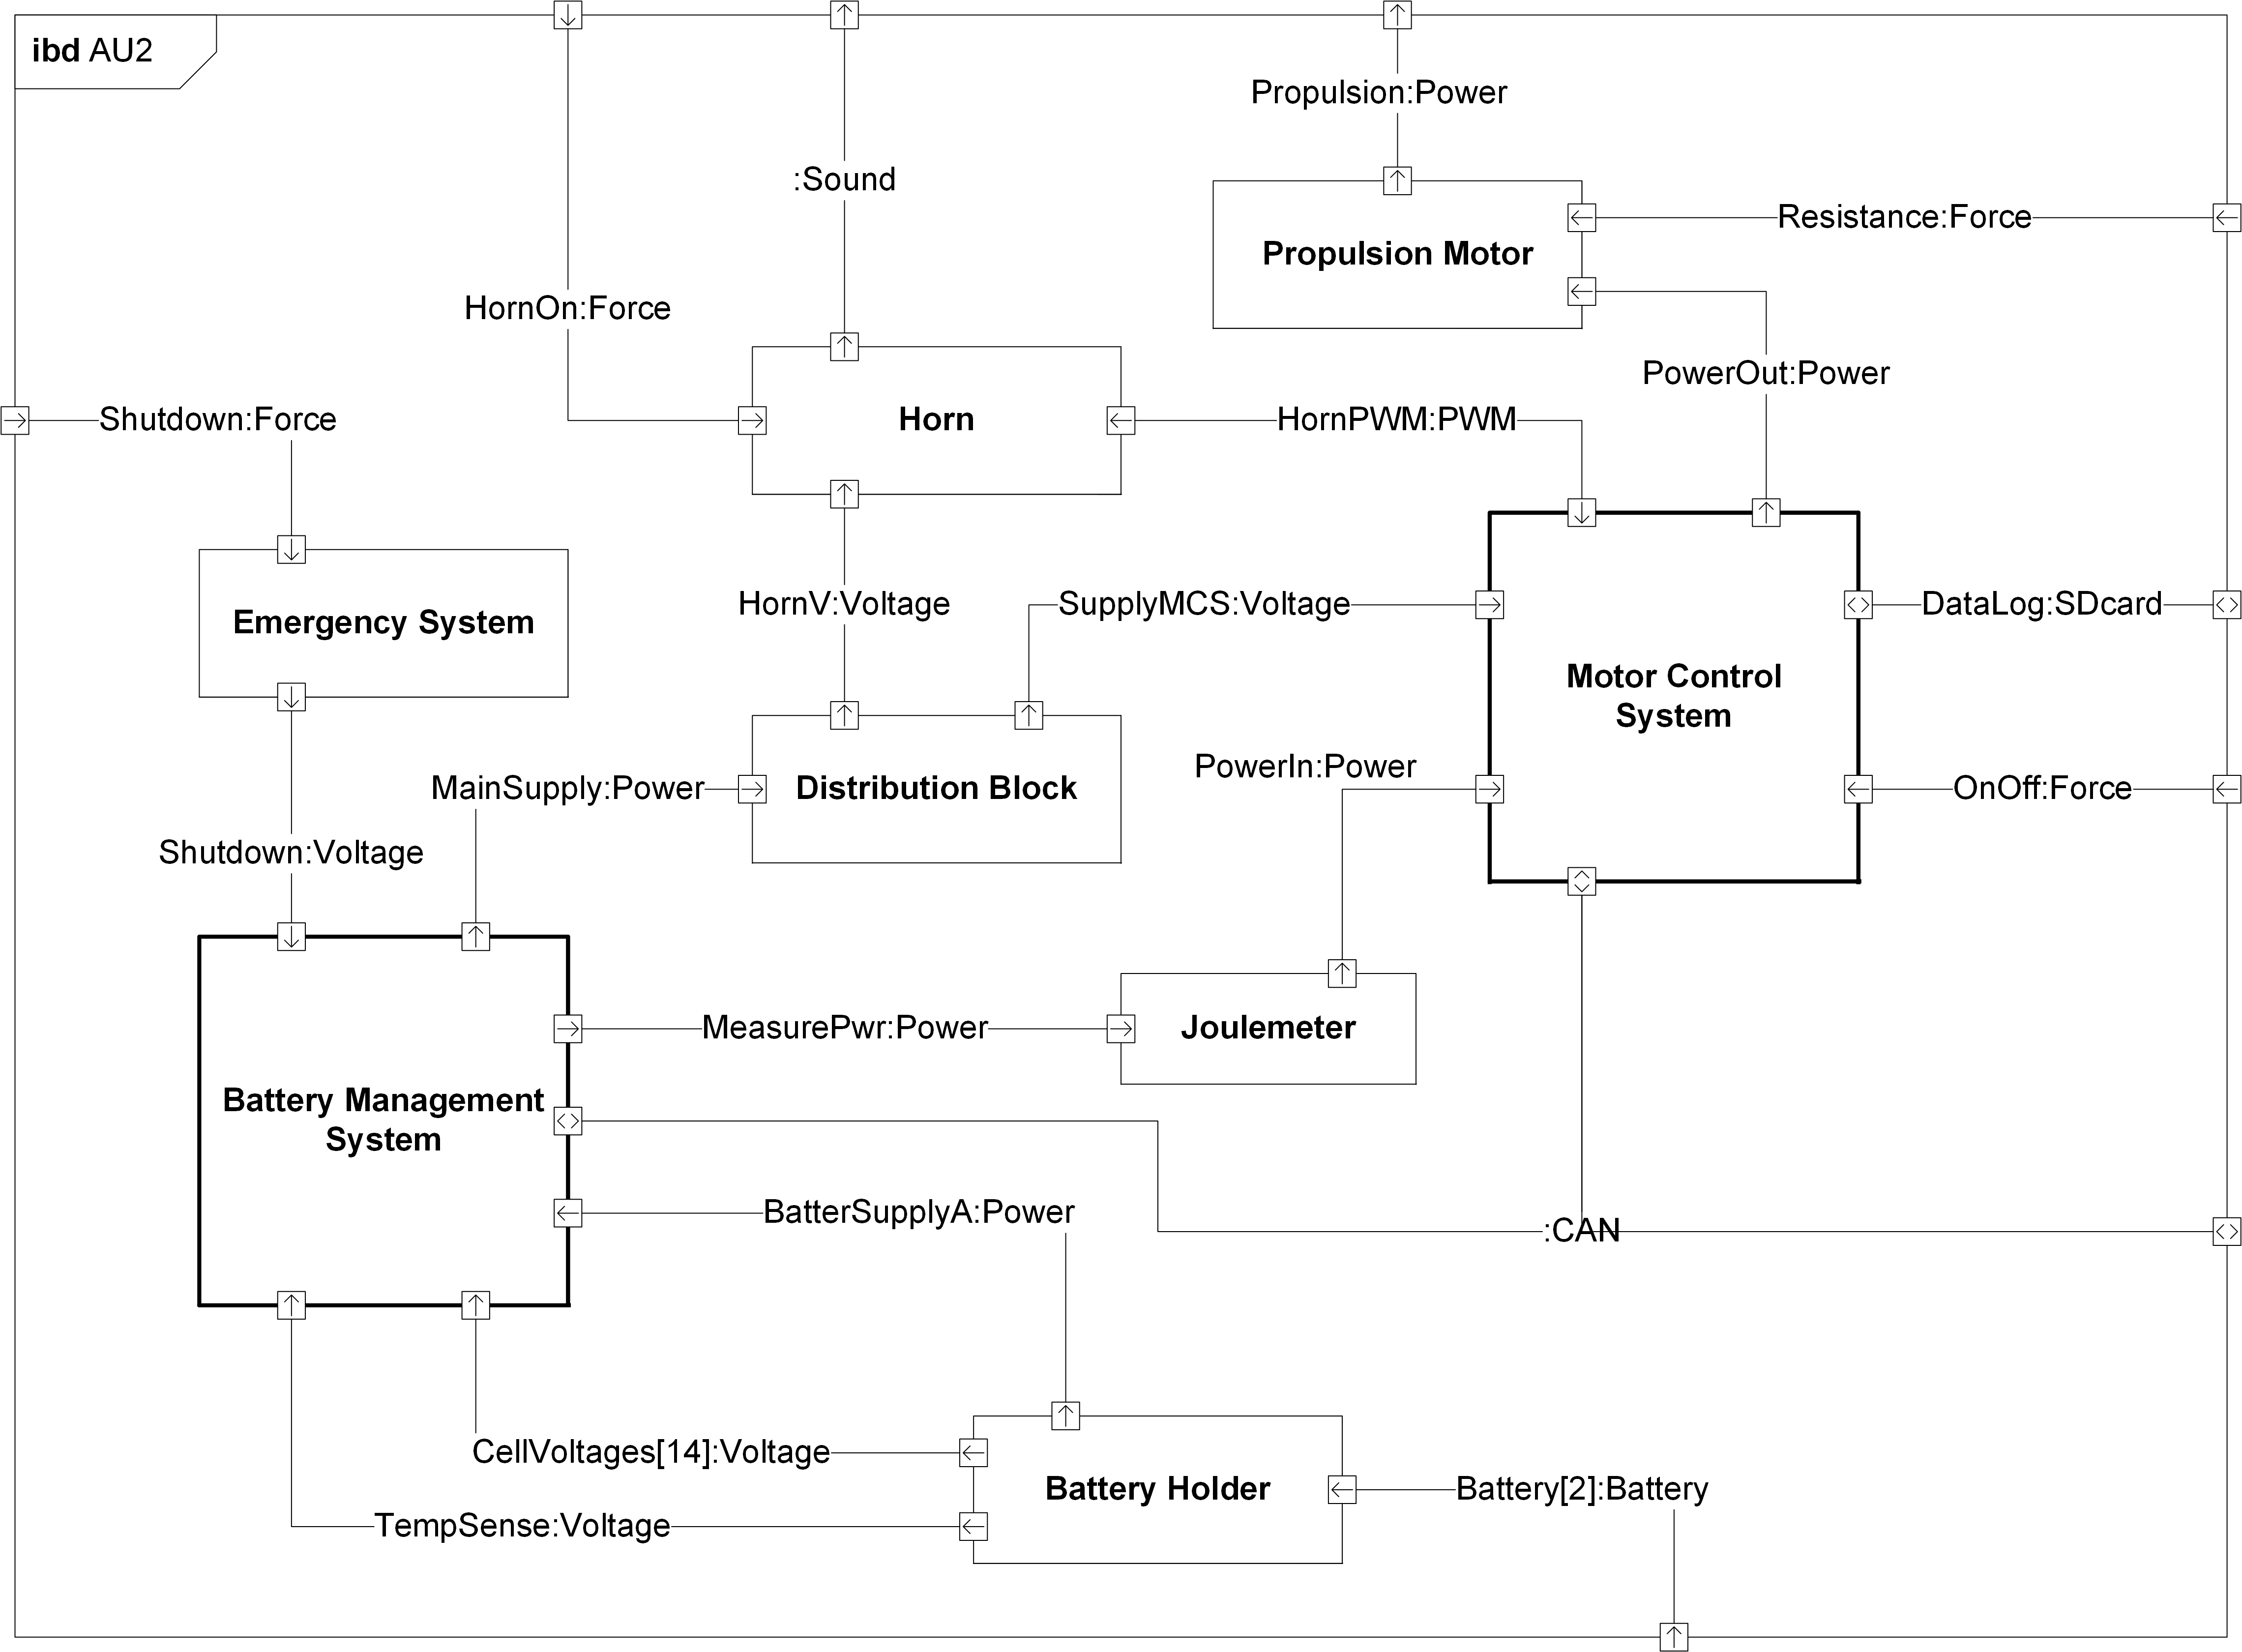
\includegraphics[width=1\linewidth]{Architecture/IBD_AU2}
	\caption{Internal Block Diagram for AU2}
	\label{fig:IBD_AU2}
\end{figure}

\begin{figure}[H]
	\centering
	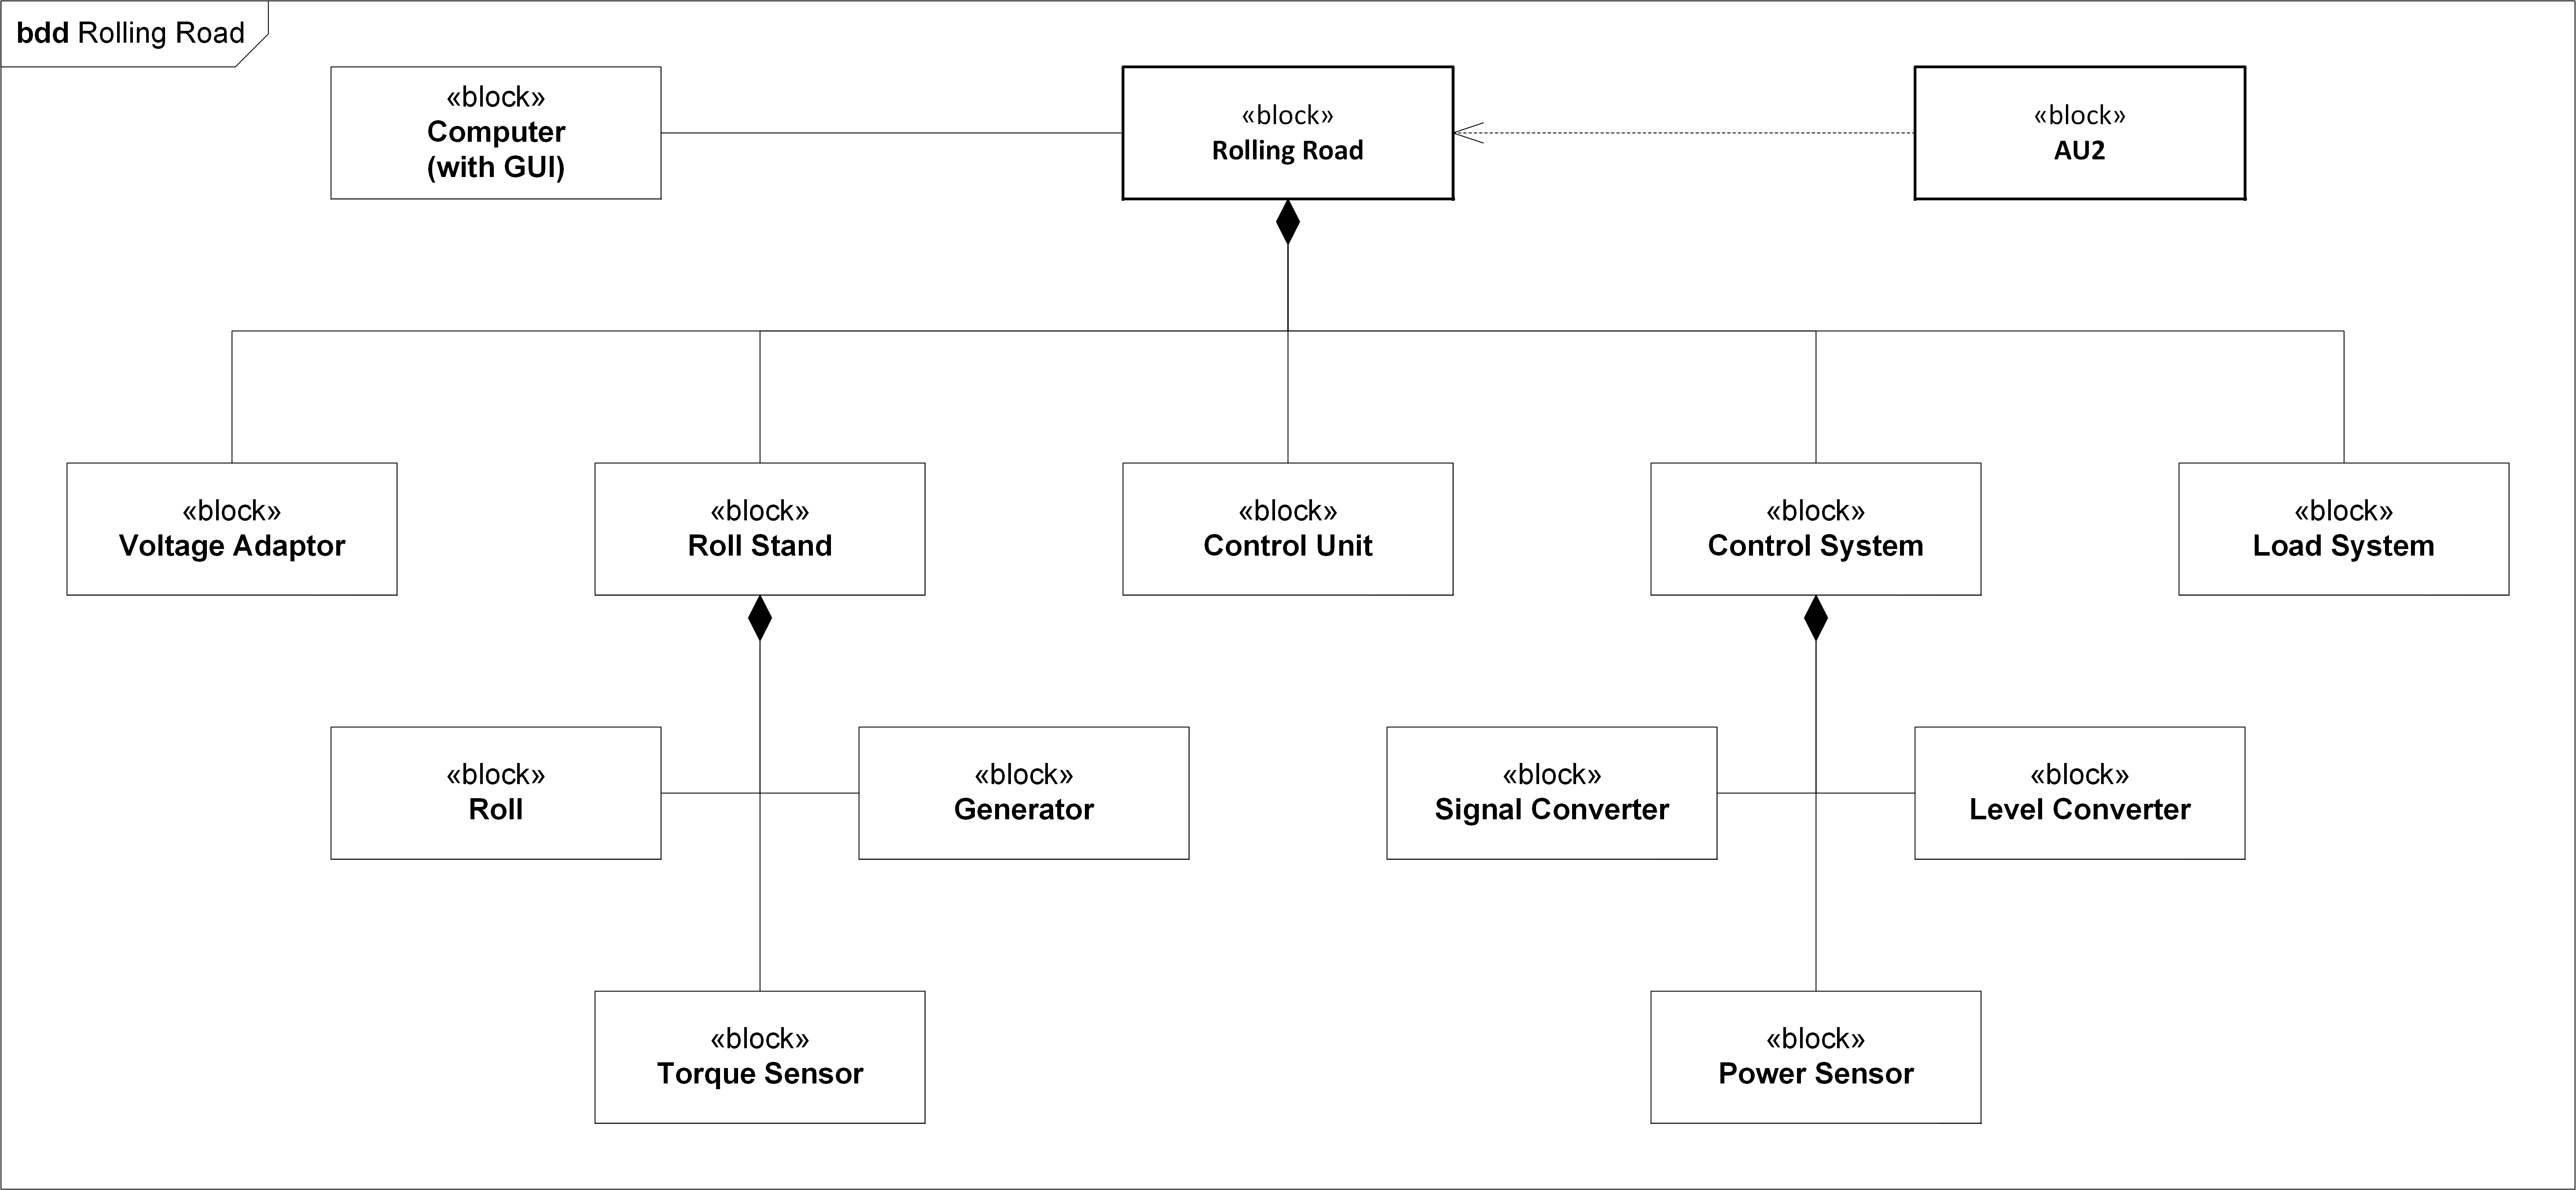
\includegraphics[width=1\linewidth]{Architecture/BDD_RR}
	\caption{Block Definition Diagram for RR}
	\label{fig:BDD_RR}
\end{figure}

\begin{figure}[H]
	\centering
	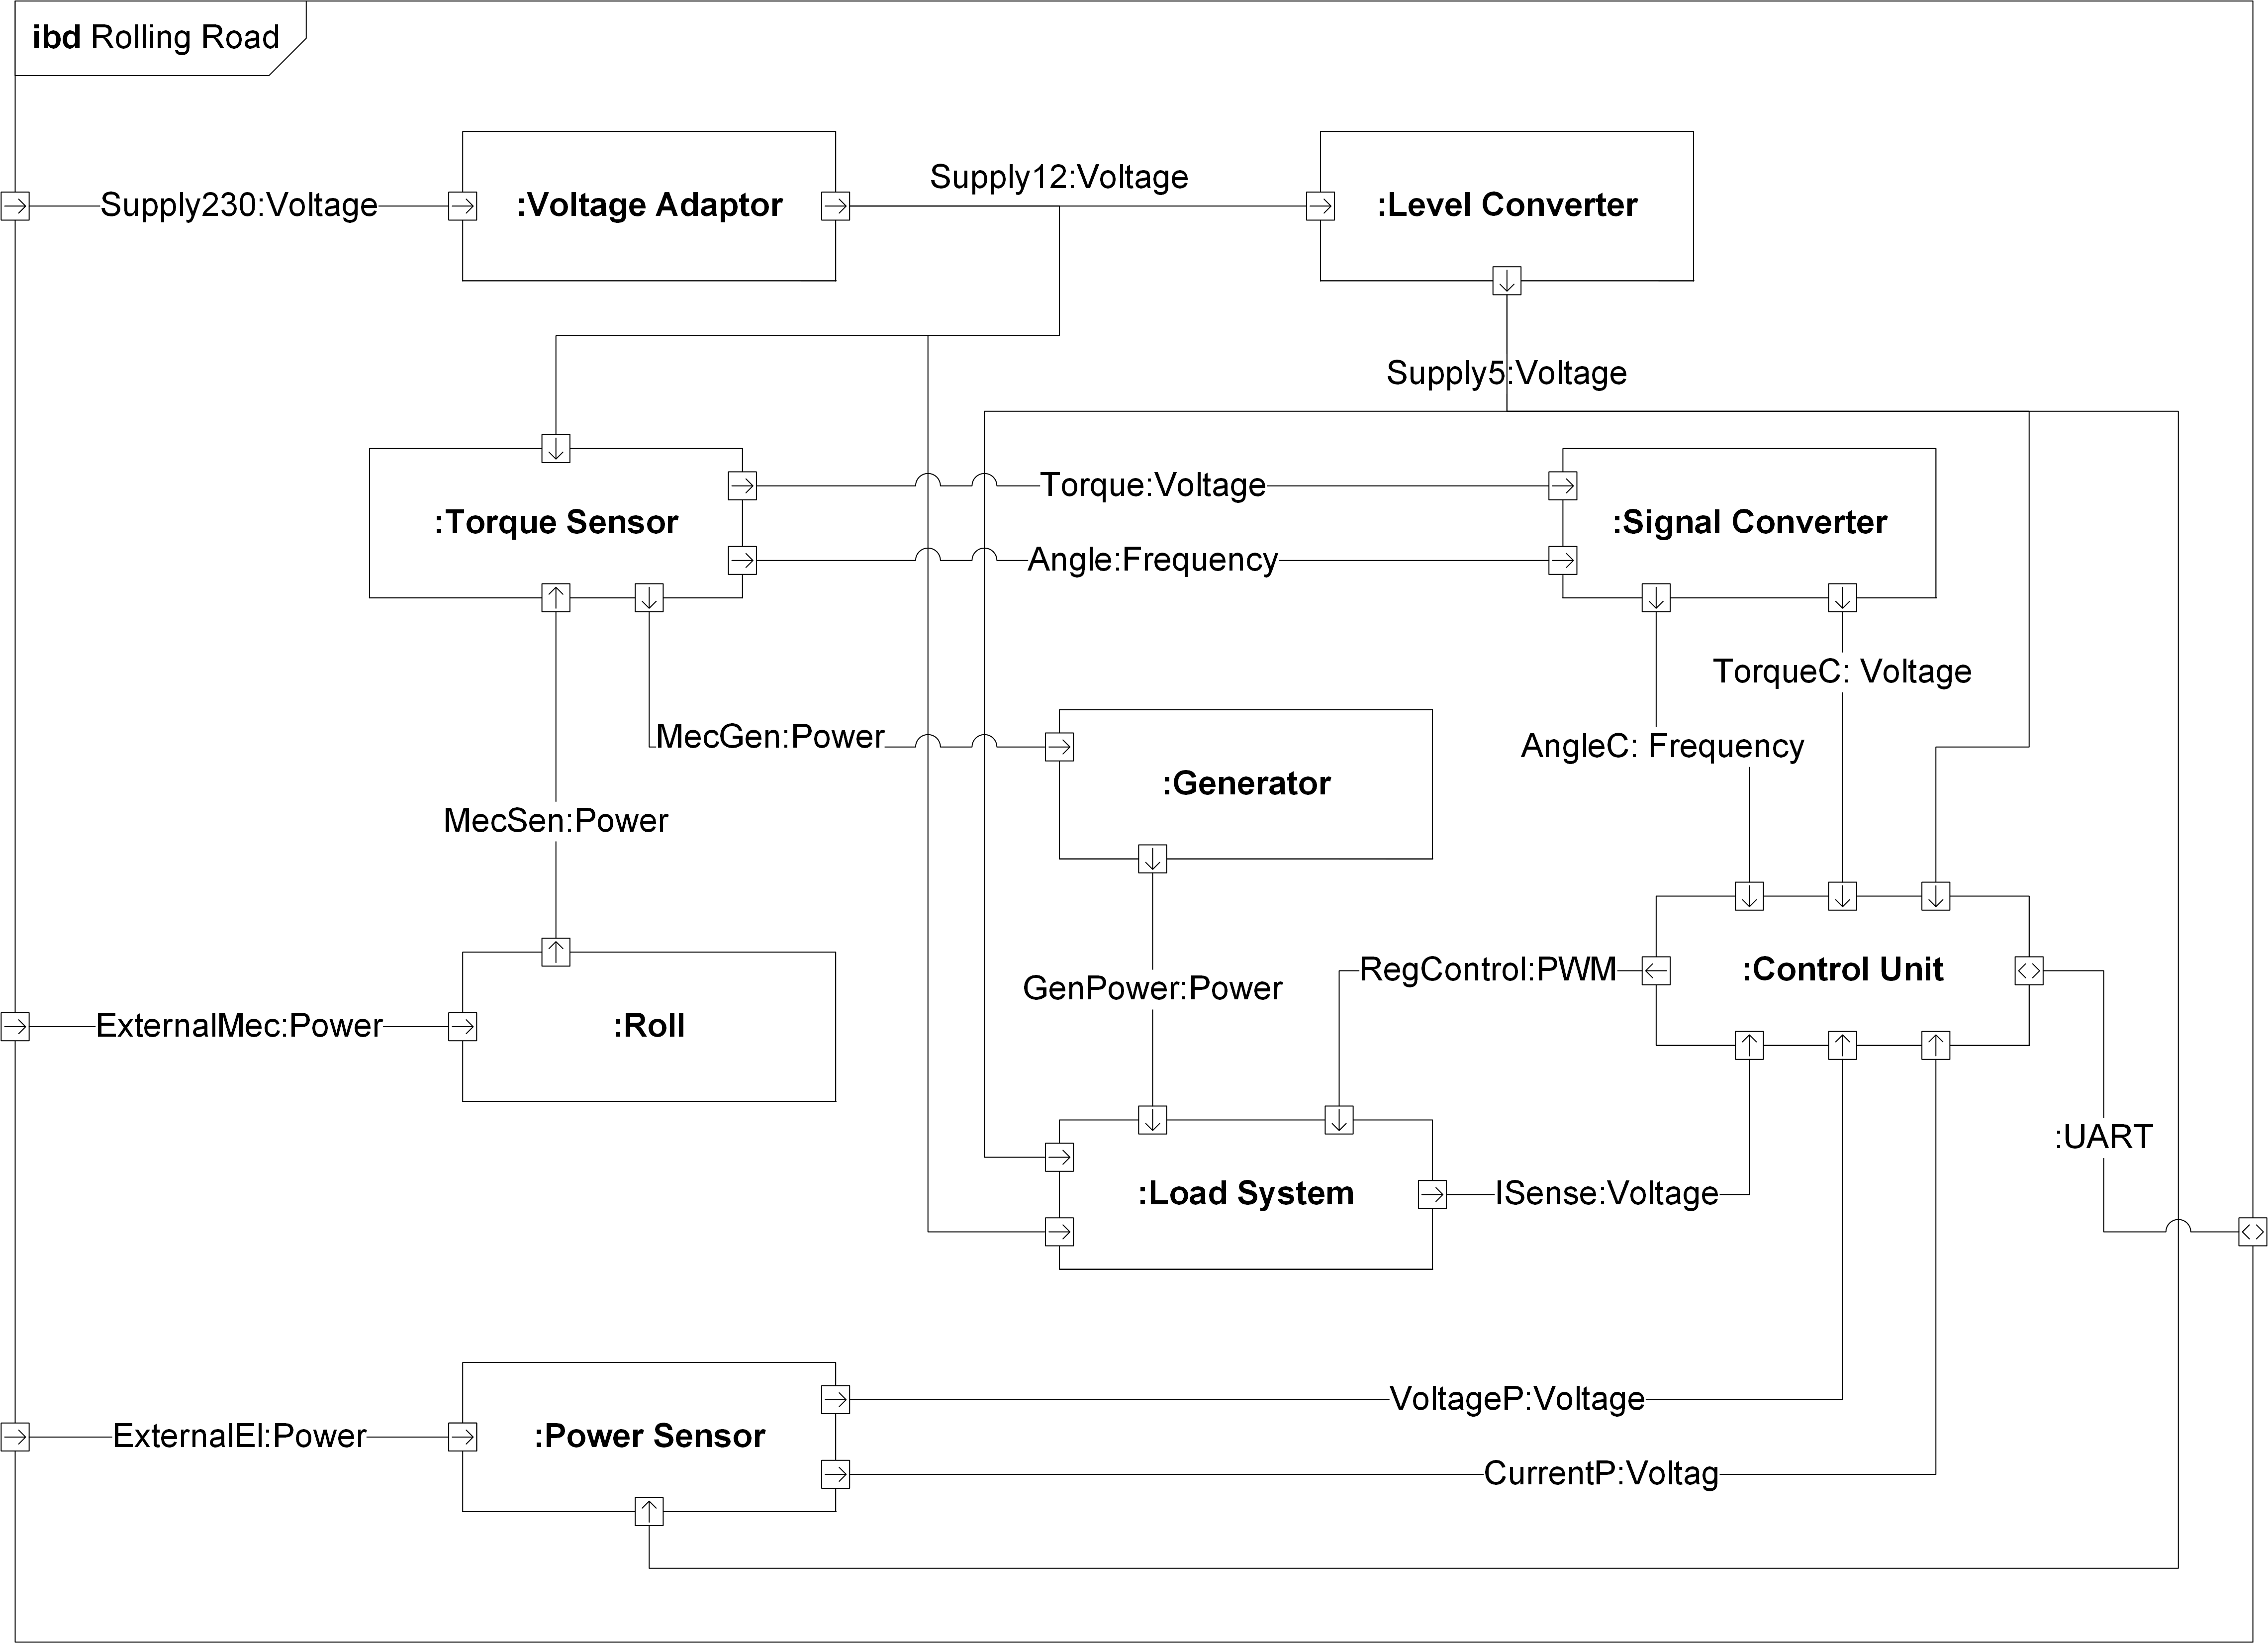
\includegraphics[width=1\linewidth]{Architecture/IBD_RR}
	\caption{Internal Block Diagram for RR}
	\label{fig:IBD_RR}
\end{figure}

The BDD and IBD for Rolling Road is seen on Figure \ref{fig:BDD_RR} and \ref{fig:IBD_RR} above. As a similar system to the Rolling Road had already been developed, the previous BDD and IBD were used to build upon. This caused the team to briefly become the reader as the previous system's diagrams were helpful in gaining an insight into the previous system. This kind of reverse-diagram-engineering led to the diagrams seen above, which differ from the previous system's diagram due to choices made during the design-phase.